% ---------------------------------------------------------------------
% HEADER
% Formålet med å legge header til et eget dokument er å garantere at
% oppsettet av dokumentene er likt for alle løsningsforslagene.
% I headeren skjer følgende:
% (1) Dokumentet blir startet
% (2) Pakker blir importert
% ---------------------------------------------------------------------
% ---------------------------------------------------------------------
% HEADER
% Formålet med header er å importere de samme pakkene i alle dokumentene.
% ---------------------------------------------------------------------

% Sett opp dokumentet. Her kan 'twoside' brukes for printing
\documentclass[12pt, a4paper]{article}

% Vi trenger utf-8 for å bruke norske bokstaver: Æ, Ø, Å
\usepackage[utf8]{inputenc}

% Vi setter babel til norsk, da får dokumentegenskaper norske titler
\usepackage[norsk]{babel}

% For å kunne bruke grafikk
\usepackage{graphicx}
\newcommand{\figwidth}{0.75}

% Matematikkpakker fra AMS - American Mathematical Society
\usepackage{amsmath, amsthm, amsfonts, amssymb, mathtools}

% For eventuelle linker, e.g. \href{URL}{text}
\usepackage{hyperref}

% For headers og footers med eventuell logo
\usepackage{fancyhdr}

% Sett marginer manuelt
\usepackage[top = 3cm, left = 3cm, right = 3cm, bottom = 3cm]{geometry}

% For enkle lister, nyttig for oppgave a), b), c), ...
\usepackage[sharp]{easylist}

% Dersom flere kolonner er ønskelig i deler av dokumentet
\usepackage{multicol}

% For luft mellom paragrafer
\usepackage{parskip}

% For logikk assosiert med logoer
\usepackage{ifthen}

% For å finne totalt antall sider
\usepackage{lastpage}

% Annet
\usepackage{enumitem}

\usepackage{polynom}% Polynomer
\polyset{style=C, div=:}

\usepackage{systeme}% Likningssystemer

% Kan brukes når noe stryker ut noe, f.eks 1/n * n, her kan man ta \frac{1}{\cancel{n}} * \cancel{n}
\usepackage{cancel}



% ---------------------------------------------------------------------
% DOKUMENTVARIABLER
% ---------------------------------------------------------------------
\newcommand{\fagkode}{R2}
\newcommand{\semesteraar}{høsten 2018}
\newcommand{\forfatter}{Markus}
\newcommand{\dokumenttittel}{Løsningsforslag -- Eksamen \fagkode, \semesteraar}


% Set til 'true' og oppgi logo dersom du vil bruke en logo
\newboolean{bruklogo}
\setboolean{bruklogo}{false}
\newcommand{\logonavn}{}

% ---------------------------------------------------------------------
% SETUP
% Formålet med å legge setup til et eget dokument å garantere at headers,
% footers, og øverste del av dokumentet er likt for alle
% løsningsforslagene.
% ---------------------------------------------------------------------
% ---------------------------------------------------------------------
% HEADER
% Formålet med setup er at dokumentene ser rimelig like ut.
% ---------------------------------------------------------------------


% ---------------------------------------------------------------------
% Alternativ font. Kommentert ut fordi Computer Modern (default) er pen
%\usepackage{kmath,kerkis}
%\usepackage[T1]{fontenc}
% ---------------------------------------------------------------------


% ---------------------------------------------------------------------
% Sett opp headers og footers
\ifthenelse{\boolean{bruklogo}}{
% Dersom logo skal brukes, sett logoen oppe til høyre med bredde 4 cm
	\rhead{\includegraphics[width=3.5cm]{\logonavn}}
}{
% Dersom logo ikke skal brukes, sett tom header
	\rhead{}
} 
\rfoot{\thepage}
\cfoot{}
\lhead{}
\lfoot{{\scriptsize Forbedringsforslag? Bidra på \url{https://github.com/tommyod/matte_eksamener_VGS}.}}
\renewcommand{\headrulewidth}{0pt}
% ---------------------------------------------------------------------


% ---------------------------------------------------------------------
% To streker under svaret
\def\answer#1{\underline{\underline{#1}}}
% ---------------------------------------------------------------------


% ---------------------------------------------------------------------
% Start selve dokumentet
% ---------------------------------------------------------------------

\begin{document}
\pagestyle{fancy}
{\bfseries \Large \dokumenttittel} \\
{ \footnotesize Laget av \forfatter 
	\hfill Sist oppdatert: \today 
	\hfill Antall sider: \pageref*{LastPage}}
\hrule
\vspace{1em}
\begin{center}
\fbox{\fbox{\parbox{.90\textwidth}{
	Dette dokumentet er open-source;
	alle kan bidra til å gjøre det bedre.
	Dersom du finner skrivefeil, matematiske feil, eller ser at forklaringene kan være bedre: ikke nøl med å sende inn en endring. 
	Du kan finne siste versjon, og bidra, på GitHub, se:
	\url{https://github.com/tommyod/matte_eksamener_VGS}
}}}
\end{center}


% ---------------------------------------------------------------------
% DOKUMENTSTART - Skriv løsningsforslaget nedenfor
% ---------------------------------------------------------------------
\section*{Del 1}
\subsection*{Oppgave 1}
\begin{easylist}[enumerate]
	\ListProperties(Style2*=,Numbers=a,Numbers1=l,FinalMark={)})

	# Vi skal derivere $f(x) = 6 \cos(2x - 1)$, og bruker kjerneregelen for å få
	\begin{equation*}
	f'(x)
	=6(-\sin(2x-1)) \cdot \frac{\text{d}}{\text{d}x}\left[2x-1\right]
	=\answer{-12\sin(2x-1)}.
	\end{equation*}

	# Vi bruker at $\cos^2(x)+\sin^2(x) = 1$ og får
	\begin{equation*}
	g'(x)=\frac{\text{d}}{\text{d}x}\left[\cos^2(x)+\sin^2(x) \right] = \frac{\text{d}}{\text{d}x}[1] = \answer{0}.
	\end{equation*}
\end{easylist}


\subsection*{Oppgave 2}
\begin{easylist}[enumerate]
	\ListProperties(Style2*=,Numbers=a,Numbers1=l,FinalMark={)})

	# Dette integralet er rett frem, vi får
	\begin{equation*}
	\int \left(2x^2-3x\right) \, \text{d}x = \answer{\frac23 x^3 - \frac32 x^2 + C}.
	\end{equation*}

	# Her bruker vi substitusjon med $u=x^2+2$.
	Da har vi at $\text{d}x = \frac{1}{2x} \, \text{d}u$ og vi får
	\begin{equation*}
	\int 4x  \cos(x^2+2) \, \text{d}x = 2\int \cos(u) = 2\sin(u) + C = \answer{2\sin(x^2+2) + C}.
	\end{equation*}

	# Vi observerer at $x^2-4=(x+2)(x-2)$ og bruker delbrøksoppspalting.
	\begin{align*}
	\int \frac{4}{x^2-4} \, \text{d}x &= \int \left(\frac{1}{x-2} - \frac{1}{x+2} \right) \, \text{d}x \\
	&= \ln|x-2| - \ln|x+2| + C = \answer{\ln \left| \frac{x-2}{x+2}\right| + C}
	\end{align*}
\end{easylist}



\subsection*{Oppgave 3}
\begin{easylist}[enumerate]
	\ListProperties(Style2*=,Numbers=a,Numbers1=l,FinalMark={)})

	# For at rekka skal konvergere må $|e^{-x}| < 1$.
	Siden $e^x>0$ for alle $x \in \mathbb{R}$, holder det med å sjekke når $e^{-x} < 1 \Longleftrightarrow e^x>1 \Longleftrightarrow x > 0$.
	Rekka konvergerer altså når \answer{$x > 0$}.
	# Vi ønsker å løse $S(x)=3$, der funksjonen $S(x)$ er summen av rekka.
	Siden $S(x)$ er en geometrisk rekke er den for alle $x>0$ slik at
	\begin{equation*}
	S(x)=\frac{1}{1-e^{-x}}=\frac{e^x}{e^x-1}.
	\end{equation*}
	Vi setter nå dette lik $3$ så får vi likningen
	\begin{equation*}
	2e^x=3 \Longleftrightarrow x = \answer{\ln\left(\frac32\right)}.
	\end{equation*}
\end{easylist}

\subsection*{Oppgave 4}

\begin{easylist}[enumerate]
	\ListProperties(Style2*=,Numbers=a,Numbers1=l,FinalMark={)})
	# Tegningen er ikke vist.
	# Vi skal finne skjæringspunktene til $\sin(x)$ og $\cos(x)$, altså løse
	\begin{equation*}
	\sin(x)-\cos(x)=0 \Longleftrightarrow \frac{\sin(x)}{\cos(x)} - 1 = 0,
	\end{equation*}
	når $\cos(x)\neq 0$. Dette forenkles igjen til $\tan(x)=1$, som skjer når $x=\frac{\pi}{4} + \pi n$, $n \in \mathbb{Z}$.
	Så skjæringspunktene er
	\begin{equation*}
	\answer{\left( \frac{\pi}{4}, \frac{\sqrt{2}}{2} \right) \text{ og } \left( \frac{5\pi}{4}, -\frac{\sqrt{2}}{{2}} \right)}.
	\end{equation*}

	# Vi finner arealet ved å løse følgende integral.
	\begin{equation*}
	\int_{\pi/4}^{5\pi/4} \left(\sin(x) - \cos(x)\right) \, \text{d}x = -\cos(x)-\sin(x)\bigg\vert_{\pi/4}^{5\pi/4} = \answer{2\sqrt{2}}
	\end{equation*}
\end{easylist}

\subsection*{Oppgave 5}
\begin{easylist}[enumerate]
	\ListProperties(Style2*=,Numbers=a,Numbers1=l,FinalMark={)})

	# Vi observerer at amplituden er $1.2$ og at perioden er $8$ sekunder.
	Jeg tolker likevektslinja til å være $0$ utifra oppgavebeskrivelsen.
	Siden $f(t)$ er på sitt høyeste når $t=0$, kan vi konkludere med at den er faseforskjøvet med $\frac{\pi}{2}$.
	Konklusjonen er
	\begin{equation*}
	\answer{f(t)=1.2\sin\left(\frac{\pi}{4}t + \frac{\pi}{2} \right)}.
	\end{equation*}


	# Her skal vi løse
	\begin{equation*}
	f(t)=0.6 \Longleftrightarrow \sin\left(\frac\pi4 t + \frac\pi2 \right)=\frac12 .
	\end{equation*}
	Dette er ekvivalent med å løse
	\begin{equation*}
	\frac\pi4 t + \frac\pi2 = \frac\pi6 + 2\pi n \qquad \text{ og } \qquad \frac\pi4 t + \frac\pi2 = \frac{5\pi}{6} + 2\pi n
	\end{equation*}
	der $n \in \mathbb{Z}$ og $t \in [0,10]$.
	Dette er igjen ekvivalent med å løse
	\begin{equation*}
	t=-\frac{4}{3} + 8n \qquad \text{og} \qquad t=\frac43 + 8n.
	\end{equation*}
	Herifra ser vi at løsningene på det ønskede intervallet er $t\in\{\frac43, \frac{20}{3},\frac{28}{3}\}$.
	Så bøyen er (strikt) 0.6 m over likevektslinja på intervallene \answer{$\left(0,\frac43 \right)$ og $\left(\frac{20}{3}, \frac{28}{3}\right)$}.
\end{easylist}


\subsection*{Oppgave 6}
\begin{easylist}[enumerate]
	\ListProperties(Style2*=,Numbers=a,Numbers1=l,FinalMark={)})

	# Observer at tangenten i $(1,-1)$ peker nedover, så alternativ $1$ ($y'=x+y$) kan ikke være rett, fordi da hadde $y'=1-1=0$ i $(1,-1)$, altså skulle tangenten vært flat.

	Hvis alternativ $2$ hadde vært korrekt skulle tangenten gått mot å stige mer og mer når $y$ nærmet seg $0$ og $x$ er liten (og positiv i dette eksempelet), for når $y'= x/ y$, og $y\to 0$, vokser helt klart $y'$. Men her går $y'$ mot å være mer og mer ``flat''.

	Eneste gjenstående alternativ er alternativ 3, så \answer{$y'=x\cdot y$ må være korrekt}.

	# Vi ser at $y'=x\cdot y \Longleftrightarrow \frac{y'}{y} = x$ .Dette er en seperabel diff.likning, vi får
	\begin{equation*}
	\int \frac{1}{y} \, \text{d}y = \int x \, \text{d}x \Longleftrightarrow \ln|y| = \frac{1}{2}x^2 + C \Longleftrightarrow \answer{y = Ce^{\frac12 x^2}}.
	\end{equation*}
\end{easylist}

\subsection*{Oppgave 7}
\begin{easylist}[enumerate]
	\ListProperties(Style2*=,Numbers=a,Numbers1=l,FinalMark={)})

	# Vi bruker at $\overrightarrow{AB} = B - A$. Svaret blir \answer{$\overrightarrow{AB} = (2,-2,-1)$ og  $\overrightarrow{AC}=(0,-1,1)$}.

	# $A(-1,1,1)$ inn i planlikningen gir $3(-1) + 2(1) + 2(1) - 1=-3+2+2-1=0$ så $A$ ligger i planet. Akkurat den samme prosessen kan brukes for å vise at $B$ og $C$ ligger i planet.

	# Vi er gitt $D(s^2-1,3s+1,10)$, $s \in \mathbb{R}$.
	Vektorene $\overrightarrow{AB}$, $\overrightarrow{AC}$ og $\overrightarrow{AD}$ utspenner et tetraeder $ABCD$ med volum $$V=\frac16 \left | (\overrightarrow{AB} \times \overrightarrow{AC}) \cdot \overrightarrow{AD}\right |.$$
	Vi regner ut at $\overrightarrow{AD}=(s^2,3s,9)$ ,og at $\overrightarrow{AB} \times \overrightarrow{AC} = (-3,-2,-2)$, så vi får at
	\begin{align*}
	V &=\frac16 \left| (-3,-2,-2) \cdot (s^2,3s,9) \right|
	=\frac{1}{6}\left|-3s^2-6s-18 \right| \\
	&=\frac{1}{6}|-3||s^2+2s+6|
	=\frac12 |s^2+2s+6|
	\end{align*}
	Observer at $s^2+2s+6=(s+1)^2+5$, så $s^2+2s+6$ er aldri negativ, og vi kan se bort ifra absoluttverditegnet.
	Derfor er funksjonen for volumet gitt ved
	\begin{equation*}
	\answer{V(s)=\frac12s^2+s+3}.
	\end{equation*}

	# Deriverer vi $V(s)$, får vi at $V'(s)=s+1$ så $V'(s)=0$ når $s=-1$.
	Observer at $V'(-2)=-1$ og $V'(0)=1$, så $(-1,V(-1))$ er et bunnpunkt.
	Det minste volumet tetraederet kan ha er altså $V(-1)=\frac12 -1 + 3 = \answer{5/ 2}$.

\end{easylist}

\subsection*{Oppgave 8}
Vi skal vise at $P(n): \enspace1^3+2^3+\dots+n^3=\frac{n^2(n+1)^2}{4}$ ved induksjon. \newline

\textbf{Basistilfellet}, $n=1$ gir venstre side lik $1^3=1$ og høyre side $\frac{1^2(1+1)^2}{4}=1$, så høyre side er lik venstre side og basistilfellet stemmer.

\textbf{Induksjonshypotesen}, $n=k$. Vi antar at formelen stemmer for $n=k$, altså at
\begin{equation*}
1^3+2^3+\dots+k^3 = \frac{k^2(k+1)^2}{4}.
\end{equation*}
\textbf{Induksjonssteget}, vi ønsker nå å vise at $P(k)\implies P(k+1)$.
\begin{alignat*}{2}
1^3+2^3+\dots+k^3+(k+1)^3 &\overset{\text{i.h}}{=} \frac{k^2(k+1)^2}{4} + (k+1)^3 \\
&= (k+1)^2\left(\frac{k^2}{4} + (k+1)\right) \\
&= (k+1)^2 \left(\frac{k^2+4k+4}{4}\right) \\
&= (k+1)^2 \left(\frac{(k+2)^2}{4}\right) \\
&= \frac{(k+1)^2((k+1)+1)^2}{4}
\end{alignat*}


\newpage
\section*{Del 2}
\subsection*{Oppgave 1}

\begin{easylist}[enumerate]
	\ListProperties(Style2*=,Numbers=a,Numbers1=l,FinalMark={)})
	# Ikke gjort.
	# Fra oppgave a) vet man allerede hvordan dette området ser ut. Skjæringspunktene fås ved å løse $f(x)=g(x)$.
	Vi får at skjæringspunktene er $\{0,2\}$. Da er
	\begin{equation*}
	M=\int_0^2 (g(x)-f(x)) \, \text{d}x = \int_0^2 (-x^4+4x^3-6x^2+4x) \, \text{d}x = \answer{\frac85}.
	\end{equation*}

	# Et skjermbilde fra Geogebra er inkludert.
	\begin{figure}[ht]
		\centering
		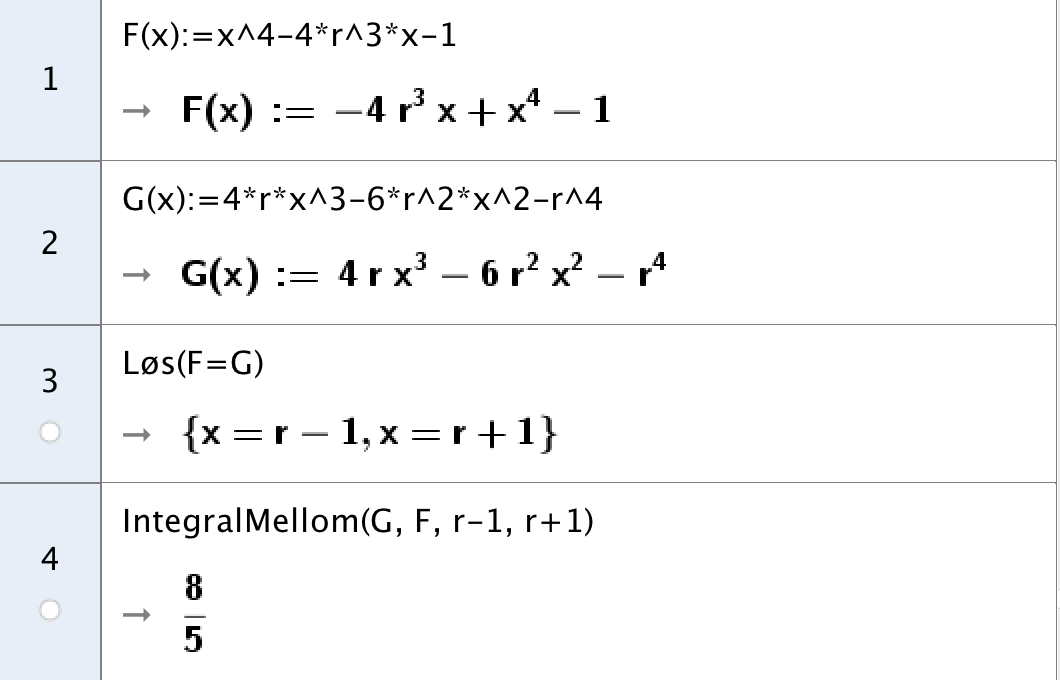
\includegraphics[width=0.7\linewidth]{ggb1.png}
	\end{figure}

	Vi ser at arealet mellom grafene er uavhengig av $r$.
\end{easylist}

\subsection*{Oppgave 2}
\begin{easylist}[enumerate]
	\ListProperties(Style2*=,Numbers=a,Numbers1=l,FinalMark={)})

	# Sentrumet i kuleflaten $K_1$ er gitt ved $(2t,1,3)$ og kulen har radius $2$.
	Formelen for en kuleflate med radius $r$ og sentrum i $(x_0,y_0,z_0)$ er gitt ved
	\begin{equation*}
	(x-x_0)^2+(y-y_0)^2+(z-z_0)^2=r^2.
	\end{equation*}
	Så for vår del blir likningen
	\begin{equation*}
	\answer{(x-2t)^2+(y-1)^2+(z-3)^2=2^2}.
	\end{equation*}

	# Kuleflaten $K_1$ vil tangere $yz$-planet når avstanden fra sentrum i $K_1$ til $yz$-planet er $2$.
	Likningen for $yz$-planet er $x=0$.
	Bruker vi nå avstandsformelen får vi at avstanden er
	\begin{equation*}
	D=\frac{|ax_1+d|}{\sqrt{a^2}} = \frac{|1\cdot2t|}{\sqrt{1^2}}=|2t|.
	\end{equation*}
	Så vi må løse $|2t|=2$, altså tangerer $K_1$ $yz$-planet når $\answer{t=\pm1}$.

	# Vi har en ny kuleflate gitt ved $K_2:\, x^2+y^2+z^2=r^2$.
	Herifra ser vi at sentrum for $K_2$ er $(0,0,0)$.
	Dersom $r=2$, vil kulene tangere hverandre når avstanden mellom sentrumene til $K_1$ og $K_2$ er $4$ (radius $K_1$ + radius $K_2$).
	Altså må vi finne når avstanden mellom $(0,0,0)$ og $(2t,1,3)$ er $4$.
	Avstanden mellom disse punktene er
	\begin{equation*}
	S=\sqrt{(2t)^2+1^2+3^2}=\sqrt{4t^2+10}.
	\end{equation*}
	Løser vi $\sqrt{4t^2+10}=4$, får vi $t^2= 3 / 2$, så $t=\pm \sqrt{3 / 2}$. Altså vil kulene tangere hverandre når $\answer{t= \pm \sqrt{3/2}}$.


	# Fra c) vet vi at avstanden mellom sentrumene, hvis $K_2$ har radius $r$, er $A(t)=\sqrt{4t^2+10}$, og at kulene tangerer hverandre når $A(t)=2+r$.
	Setter vi $A(t)=2+r$, får vi likningen
	\begin{equation*}
	4t^2+10=4+4r+r^2 \Longleftrightarrow t^2 = \frac14r^2+r-\frac{3}{2}.
	\end{equation*}
	Siden $t^2\geq0$ for alle $t \in \mathbb{R}$, må vi ha at $\frac14r^2+r-\frac{3}{2}\geq0$.
	Denne likningen har to løsninger, der henholdsvis en er positiv, nemlig $r=\sqrt{10}-2$.
	Altså er $\answer{r=\sqrt{10}-2}$ den minste verdien som sørger for at de to kulene tangerer.
\end{easylist}


\subsection*{Oppgave 3}
\begin{easylist}[enumerate]
	\ListProperties(Style2*=,Numbers=a,Numbers1=l,FinalMark={)})

	# Hvis bedriften klarer å nå målet blir utslippet i 2018 lik 20 000 tonn, i 2019 lik $20 000\cdot(0.85)$, i 2020 vil den være $(20000\cdot 0.85)\cdot 0.85 = 20000 \cdot 0.85^2$.
	Vi ser at mønsteret danner en geometrisk rekke, så fra 2018 til 2027 blir summen av utslippene lik
	$$\sum_{n=0}^9 20000\cdot 0.85^n \approx \answer{107083.4 \, \text{ (tonn)}}$$

	#  Om den andre bedriften vet vi at utslippene deres over $2018-2027$ er
	\begin{equation*}
	S(r)=\sum_{n=0}^{9} 30000\cdot r^n.
	\end{equation*}
	Vi er bedt å finne $r$ slik at bedriften i a) og denne bedriften slipper ut like mye.
	Formelen for summen av en geometrisk rekke lar oss omskrive $S(r)$ til
	\begin{equation*}
	S(r)=30000 \left(\frac{1-r^9}{1-r}\right).
	\end{equation*}
	Settes $S(r)$ lik svaret i a) (dette kan man for eksempel gjøre i CAS), fås $r\approx 0.74$, så bedriften må \answer{redusere utslippene hvert år med omtrent $74 \, \%$} for at bedriftene skal slippe ut det samme over samme periode.
\end{easylist}

\subsection*{Oppgave 4}
\begin{easylist}[enumerate]
	\ListProperties(Style2*=,Numbers=a,Numbers1=l,FinalMark={)})
	# Tallet $3.2$ sier oss at det renner inn $3.2$ liter vann i tanken per min, $0.14$ sier oss at det renner ut $14 \, \%$ av innholdet i tanken per minutt og $y(0)=200$ sier oss at det var $200$ liter vann i tanken til å starte med.

	# Dette er en lineær første ordens diff.likning
	\begin{equation*}
	y'+0.14y=3.2,
	\end{equation*}
	og integrerende faktor er $e^{\int 0.14 \, \text{d}t} = e^{0.14t}$.
	Vi løser likningen ved å skrive
	\begin{alignat*}{1}
	e^{0.14t}\left(y'+0.14y\right) &= 3.2e^{0.14t} \\
	\left(ye^{0.14t} \right)' &= 3.2e^{0.14t} \\
	\int \left(ye^{0.14t} \right)' \, \text{d}t &= \int 3.2e^{0.14t} \, \text{d}t \\
	ye^{0.14t} &= \frac{160}{7}e^{0.14t} + C \\
	y &= \frac{160}{7} + Ce^{-0.14t}
	\end{alignat*}
	Med initialverdibetingelsen $y(0)=200$ fås $C=200-\frac{160}{7} = \frac{1240}{7}$, og vi får
	\begin{equation*}
	\answer{y(t) = \frac{160}{7} + \frac{1240}{7}e^{-0.14t}}.
	\end{equation*}


	# Vi regner ut $y(20) \approx \answer{33.63 \enspace \text{(liter)}}$.

	# Utifra opplysningene danner vi oss diff.likningen $y'=1.5-ky$ for en $k \in \mathbb{R}$, der $y(0)=0$.
	Denne diff.likningen kan løses likt som i b) og vi får den generelle løsningen
	\begin{equation*}
	y(t)=\frac{1.5}{k} + Ce^{-kt}.
	\end{equation*}
	Med initialverdibetingelsen $y(0)=0$ fås
	\begin{equation*}
	y(t)=\frac{1.5}{k} - \frac{1.5}{k}e^{-kt}.
	\end{equation*}
	Videre vet vi at mengden vann i tanken vil stabilisere seg på 10L etterhvert, med andre ord er
	\begin{equation*}
	\lim_{t \to \infty} \left[\frac{1.5}{k} - \frac{1.5}{k}e^{-kt}\right] = 10.
	\end{equation*}
	Vi kan herifra konkludere at $k=\dfrac{1.5}{10}$.
	Derfor er funksjonen vår er gitt ved
	\begin{equation*}
	y(t)=10-10e^{-0.15t}.
	\end{equation*}
	Og etter 20 minutter vil da derfor være
	\begin{equation*}
	y(20)\approx \answer{9.50 \enspace (\text{liter i tanken})}.
	\end{equation*}
\end{easylist}

\end{document}
